\documentclass[10pt,conference]{ieeeconf}
\usepackage{amsmath}
\usepackage{amssymb}
\usepackage{cite}
\usepackage{graphicx}
\usepackage{mathnotation}
\usepackage{oubraces}
\usepackage[ruled]{algorithm2e}

\makeatletter
\def\endthebibliography{%
  \def\@noitemerr{\@latex@warning{Empty `thebibliography' environment}}%
  \endlist
}
\makeatother

\DeclareRobustCommand{\groupderiv}[1]{\accentset{\scriptstyle\circ}{#1}}
\renewcommand{\localconn}{\mixedconn}
% taken from IEEEtran
\DeclareRobustCommand*{\IEEEauthorrefmark}[1]{\raisebox{0pt}[0pt][0pt]{\textsuperscript{\footnotesize\ensuremath{\ifcase#1\or *\or \dagger\or \ddagger\or%
    \mathsection\or \mathparagraph\or \|\or **\or \dagger\dagger%
    \or \ddagger\ddagger \else\textsuperscript{\expandafter\romannumeral#1}\fi}}}}
\SetKwComment{Comment}{//}{}

\title{Kinematic Path Planning Under Uncertainty}
% Optimal Choice of Robot Intrinsic Dimension
\author{
    \authorblockN{
        Capprin Bass\IEEEauthorrefmark{1},
        Neha Pusalkar\IEEEauthorrefmark{2}, and
        Brett Stoddard\IEEEauthorrefmark{3}
    }
    \authorblockA{  
        Collaborative Institute for Robotics and Intelligent Systems (CoRIS),
        Oregon State University\\Corvallis, Oregon \\
        Email: \{\IEEEauthorrefmark{1}basscap,
        \IEEEauthorrefmark{2}pusalkan,
        \IEEEauthorrefmark{3}stoddabr\}@oregonstate.edu
    }
}

\begin{document}

\maketitle

\begin{abstract}
    Recently in the robotics industry, companies construct certain research robots from cheaper components, lowering the barrier of entry to study robot systems.
	These systems pose a challenge from a planning and control standpoint, as uncertainty in actuation and sensing propagates into the trajectory of the robot.
	In this paper, we present a novel method of expressing joint space uncertainty in the task space, respecing system kinematics.
	We cast this expression for uncertainty as a pathlength metric, reflecting uncertainty accrued over a path.
	Finally, we use our covariant pathlength metric as a heuristic for path planning, producing paths for a planar manipulator that minimize uncertainty.
\end{abstract}

\section{Introduction}\label{sec:introduction}
% historic robots
	% powerful actuators
	% precise encoders
	% task space plans can be followed using simple kinematics or dynamics
Modern industrial robots are built to be controlled using kinematic and dynamic principles.
Many systems take advantage of powerful actuators, precise sensors, and fast computers to make software control tenable, using these mechanical models.
Task space path plans can be followed with PID control on top of inverse kinematics or dynamics; the result is a robust stack of methods that has seen widespread use in industry \cite{something?}
However, this approach literally comes at a cost: industrial robots range in price from tens to hundreds of thousands of dollars \cite{pricing}

% newer robots
	% goal of lower cost / barrier to entry
	% cheaper actuators + hardware
	% more sources of error, so uncertainty ought to be accounted for in planning & control
A recent trend in robotics is the construction of lower cost systems, often with the goal of a lower barrier to entry in robotics research.
Some current examples of robots built with this goal include Hello Robot's Stretch \cite{stretch}, Pollen Robotics' Reachy \cite{reachy} and others, as well as a universe of hobby and DIY robots.
These systems often may be characterized as the antithesis of current industrial robots: inexpensive actuators, sensors, and computers are chosen on purpose to keep cost low.
The relative imprecision of constitutent components makes control of these systems a challenge.
Uncertainty must be built into models for system behavior, and ought to be accounted for when designing motion plans.

% here, provide a simple approach to represent first order error in robot systems, based on system kinematics
	% take covariance matrix defined on joint space as first order representation of error
	% use first order kinematic map (jacobian) to represent variance in the task space
	% provide Jinv expression
	% use task space variance as a metric on path length
	% incorporate in path planning to find low-variance paths between points
In this paper, we address the need for uncertainty-aware path planning with a novel approach, taking advantage of first-order system kinematics to represent uncertainty at the end effector.
Unlike many previous approaches \cite{previous work?}, our method respects the mapping between joint space uncertainty and the task space, which provides an intuitive representation of uncertainty at any configuration.
We use the covariance between actuators to represent uncertainty in the joint space and map it up to the task space using an \textit{inverse pullback} operation:
\begin{equation}
	M = \left(J^\dagger\right)^T \Sigma \; J^\dagger,
\end{equation}
where $M$ is the uncertainty expressed in the task space, $J$ is the jacobian of the manipulator, and $\Sigma$ is the joint-space defined covariance.
The task space uncertainty $M$ may be used as a length metric for paths defined in the task space; it reflects the uncertainty accrued by taking a given path.
We demonstrate our covariant pathlength metric as a heuristic for path planning, producing paths that respect system uncertainty.

% roadmap
The remainder of this paper is organized as follows.
In \S\ref{sec:background}, we review the relevant background in kinematics, geometry, and path planning.
In \S\ref{sec:methods}, we describe how the covariance matrix is mapped into the task space, and how uncertainty is accounted for in path planning.
In \S\ref{sec:analysis}, we demonstrate our method on a planar manipulator, generating low-uncertainty paths.
In \S\ref{sec:conclusion}, we make final remarks and comment on future work.

\section{Background}\label{sec:background}
\subsection{Model and Kinematic Map}
% define joint space, task space
When studying robot systems, we usually distinguish between the joint space and the task space.
The joint space $\Theta$ refers to the set of actuator configurations, and the task space $G$ refers to the set of end effector or baseframe configurations.
In this paper, we focus on revolute manipulators in the plane; this implies that $\Theta = S^N$, where $N$ is the number of joints, and $G = SE(2)$.

% jacobian maps between tangent spaces
The robotics community uses a number of methods to move between the joint space and the task space.
These are often referred to as forward kinematics, inverse kinematics, and their dynamic counterparts.
The most important mapping in the context of this paper is the Jacobian, which maps between tangent spaces. In our case, for $\theta \in \Theta$, this is:
\begin{equation}
    J(\theta): T_\Theta \to T_G.
\end{equation}
The Jacobian may be interpreted as a first order kinematic map; it linearly maps velocity in the joint space at a given configuration to velocity in task space.
For $g\in G$ and $\theta \in \Theta$, this is:
\begin{equation}\label{eqn:jforward}
    \dot{g} = J(\theta)\dot{\theta}.
\end{equation}

\subsection{Bilinear Forms}
% how to do inverse pullback of a bilinear form
Here, the Jacobian is used to map velocity-dependent quantities (represented as bilinear forms) from the joint space to the task space.
Bilinear forms are usually defined as symmetric or skew-symmetric matrices $\Omega$:
\begin{equation}
    \Omega =
    \begin{bmatrix}
        \Omega_{11} & \Omega_{12} & \Omega_{13} & \cdots \\
        \pm\Omega_{12} & \Omega_{22} & \Omega_{23} & \cdots \\
        \pm\Omega_{13} & \pm\Omega_{23} & \Omega_{33} & \cdots \\
        \vdots & \vdots & \vdots & \ddots
    \end{bmatrix},
\end{equation}
and operate on velocities $\dot{\theta}_1, \dot{\theta}_2$ using matrix multiplication:
\begin{equation}\label{eqn:bil}
    \Omega(\dot{\theta}_1, \dot{\theta}_2) = (\dot{\theta}_1)^T \Omega \; \dot{\theta}_2.
\end{equation}
The key benefit to this representation is that the Jacobian may be used to relate forms defined on the joint space to quantities in the task space.
From (\ref{eqn:jforward}), we relate task space velocities to joint space velocities:
\begin{equation} \label{eqn:jinv}
    \dot{\theta} = J^\dagger\dot{g},
\end{equation}
where $J^\dagger$ refers to the pseudoinverse of the Jacobian, and respects the fact that $J$ is not always invertible.
Now, (\ref{eqn:jinv}) is applied to (\ref{eqn:bil}) to \textit{pullback} workspace velocities by the inverse of the kinematic map:
\begin{equation}
    \Omega(\dot{g}_1, \dot{g}_2) = 
    \overunderbraces{&\br{2}{(\dot{\theta}_1)^T}& &\br{2}{\dot{\theta}_2}}{
        &(\dot{g}_1)^T\;&
        (J^\dagger)^T&
        \;\Omega^\Theta
        &J^\dagger \;&\dot{g}_2&
    }{&&\br{3}{\Omega^G}&&}.
\end{equation}
Bilinear forms have a broad set of applications; in this paper, we use them in two specific ways.
The first is to define covariance over the joint space, as a first order estimate for uncertainty.
The second is to define a Riemannian metric, which measures distance over a space, and is essential for alternate definitions of pathlength for planning.

\subsection{Covariance Matrix}
In probability and statistics, variance $\sigma$ measures the expected (or average) deviation from the mean in a random variable.
As an extension, \textit{covariance} $\Sigma$ between two (or more!) random variables measures how each effects the other, i.e. how correlated the two distributions are.
As an example, for random variables $X$ and $Y$, the covariance $\Sigma$ may be written as a matrix,
\begin{equation}
    \Sigma =
    \begin{bmatrix}
        \sigma_{XX} & \sigma_{XY} \\
        \sigma_{YX} & \sigma_{YY}
    \end{bmatrix},
\end{equation}
where the diagonal $\sigma_{ii}$ terms refer to the variance of each distribution, and the off-diagonal $\sigma_{ij}$ terms refer to the contribution of the \textit{other} distribution towards variance.

Due to the shared properties\footnote{
    Specifically, the important shared properties between covariance and bilinear forms are biliniarity, symmetry, positive semi-definiteness.
} between covariance and general bilinear forms, we may interpret covarariance as a bilinear form.
When we do so, \textit{vectors} are linear combinations of random variables, and matrix multiplication yields the variance of said linear combination.
For a linear combination vector $c$, the variance $\sigma(c)$ is
\begin{equation}
    \sigma(c) = c^T \Sigma \; c.
\end{equation}

We now describe Riemannian metrics, a related application of bilinear forms, generally defining distance.

\subsection{Riemannian Metrics}
Formally, a Riemannian metric defines an inner product on the tangent space (here, $T_\Theta$ or $T_G$).
The inner product can be thought of as a generalization of the dot product: it measures (by some choice of measurement) the similarity of two vectors.
A useful consequence of the inner product is that a vector may be measured against \textit{itself} to provide a measure of length.

On a broader scale, lengths are measured by integrating the metric (represented as a bilinear form) over a path definition.
For a metric $M$, path parametrization $\phi(t)$, and location $x(t)$, the weighted length $L_\phi$ is
\begin{equation}\label{eqn:length}
    L_\phi = \int_\phi \left((\dot{x})^T M(x)\;\dot{x}\right)^\frac{1}{2} d\phi.
\end{equation}
In the discrete case, weighted length of a path with $n$ segments is given by
\begin{equation}
    L_\phi = \sum_i^{n-1} \left(\Delta x_{i, i+1}^T M(x_i) \Delta x_{i, i+1}\right)^\frac{1}{2},
\end{equation}
as we weight the length of each segment $\Delta x_{i,i+1}$ by the metric $M$.

In this paper, a Riemannian metric is used to define a custom measure of distance.
Metric distance applied to a path planning algorithm can produce optimal paths with respect to our own choice of distance.

\subsection{Path Planning}
Path planning is a rich area of study, most of which is outside the scope of this paper.
However, most planners can take advantage of a number of distance measures to compare candidate paths \cite{something?}; classic examples include Euclidean distance or Manhattan distance.
Here, we use a simple path planner, A* search, to find shortest paths under metric distance.

% NEHA: brief explanation of A* search?
\noindent\textbf{[Insert explanation of A* search here]}

\section{Covariance as a Pathlength Metric}\label{sec:methods}
Here, we draw on the methods introduced in \S\ref{sec:background} to represent uncertainty respecting system kinematics.
We briefly express our method using the relevant mathematics, and explain algorithmic implementation.
We integrate our approach with path planning, generating uncertainty-aware motion plans.

\subsection{Kinematic Mapping of the Covariance Matrix}
% definition of covariance matrix
The key innovation of this work is casting covariance as a pathlength metric.
We define uncertainty in the joints of a system using a covariance matrix defined on the joint space.
The variance $\sigma$ generated by a set of joint motions $\dot{\theta}$ is given by the covariance matrix $\Sigma$ as
\begin{equation}
    \sigma(\dot{\theta}) = (\dot{\theta})^T \Sigma \; \dot{\theta}.
\end{equation}

% inverse pullback of the covariance matrix
By interpreting covariance $\Sigma$ as a bilinear form, we can represent it on the task space.
We map $\Sigma$ from the joint tangent space $T_\Theta$ to the task tangent space $T_G$ using an inverse pullback:
\begin{equation}
    \sigma(\dot{g}) =
    \overunderbraces{&\br{2}{(\dot{\theta})^T}& &\br{2}{\dot{\theta}}}{
        &(\dot{g})^T\;&
        (J^\dagger)^T&
        \;\Sigma\;
        &J^\dagger \;&\dot{g}&
    }{&&\br{3}{M}&&}
    \longrightarrow
    M(\theta) = (J^\dagger)^T \Sigma \; J^\dagger,
\end{equation}
which can be written simply as
\begin{equation}
    \sigma(\dot{g}) = (\dot{g})^T M \; \dot{g}.
\end{equation}

% interpretation in the task space (figure)
The task space covariance $M(\theta)$ can be interpreted in a similar way to a manipulability ellipsoid.
For any configuration $\theta$, covariance $M(\theta)$ can be drawn as an ellipse at the end effector of the manipulator, where the major axis encodes the direction generating the most variance.
Fig. \ref{fig:samples} demonstrates this empirically, for joint samples drawn from the multivariate normal distribution, pulled back through the system kinematics.
\begin{figure}[tb]
    \centering
    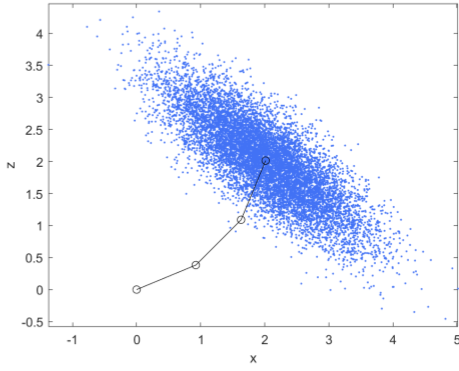
\includegraphics[width=0.9\linewidth]{images/gaussian_firstorder.png}
    \caption{
        Joint space multiviariate normal distribution, pulled back through first order system kinematics.
        Resulting work space samples are lie in an ellipse, centered about the end effector.
    }
    \label{fig:samples}
\end{figure}

% use as a riemannian metric
We now interpret covariance as a Riemannian metric on the task space.
As in (\ref{eqn:length}), the aggregate variance (or, uncertainty) $\sigma_\phi$ generated by a path $\phi(t)$ in the task space can now be written as
\begin{equation}\label{eqn:metriclength}
    \sigma_\phi = \int_\phi \left((\dot{g})^T M(\theta(t))\;\dot{g}\right)^\frac{1}{2} d\phi.
\end{equation}
We use this measure for length to perform path planning in the task space, selecting paths that minimize accrued uncertainty.

\subsection{Planning Under Uncertainty}
% given a task space path, how do we construct the covariance matrix?
For planning to take advantage of the covariant metric, we require the configuration of the manipulator at each point along the path.
We then compute lengths using (\ref{eqn:metriclength}), used both to compute path and heuristic lengths.
This process is described here, as well as in Algorithm \ref{alg:planning}.
\SetKw{Kw}{in}
\begin{algorithm}[tb]\label{alg:planning}
    \caption{Computation of Metric-Weighted Pathlengths}
    \KwIn{Arm geometry $geom$, Path discretization $path$, Covariance $\Sigma$}
    \KwOut{Pathlength $len$}

    $len \gets 0$\\
    \For{lastPoint, point, nextPoint \Kw path}{
        \Comment{use Newton-Rhapson for arm shape}
        $shape \gets$ inverseKinematics$(lastPoint, point)$\\
        $J \gets $ bodyJacobian$(geom, shape)$\\
        \Comment{compute metric}
        $M \gets (J^\dagger)^T \Sigma J^\dagger$\\
        \Comment{measure segment vector}
        $g = (nextPoint - point)$\\
        $len \gets len + \left((g)^T M\; g\right)^\frac{1}{2}$
    }
    \Return{len}
\end{algorithm}

% perform newton-rhapson inverse kinematics at each point to get the Jacobian
% compute covariance matrix at each point
% use cov mat to compute length (show math)
% include algorithm environment
% use as heuristic/pathlength in planning algorithms

\section{Results and Analysis}\label{sec:analysis}

\section{Conclusion}\label{sec:conclusion}

\bibliographystyle{./IEEEtran}
\bibliography{./IEEEabrv,./gm-references/gm.bib}

\end{document}
